\graphicspath{{Images/}}

\section{Tester}

De forma geral, no Tester, corre um \textit{script} a partir de um botão (figura 7). E mais 3 scripts quando se edita uma célula específica (figura 8).

\subsection{Impressão de Escala}
Através do botão "TESTE" inicia-se o \textit{script} "insertRow" (Tester\_04\_Get\_printTable). Este \textit{script} faz uma requisição externa HTTP GET. Esta função tem o propósito de permitir aos alunos terem acesso à folha, enquanto o \textit{script} corre. Caso isto não aconteça, não seria possível haver disposição das escalas nesta folha.

Através da função doGet é chamada a função "printTable" (Tester\_04\_printTable). Este script tem como objetivo mostrar quando é que o aluno irá fazer o seu próximo serviço. A primeira parte verifica se o aluno está a realizar uma troca, caso seja verdade, a escala será colocada na primeira tabela. Na segunda parte, consoante a verificação feita na primeira parte do programa, a escala efetiva é colocada no primeiro local ou no segundo (fig.).

\subsection{Tabela de Trocas}

\subsubsection{Verificar}
Após colocar os NIP's para as trocas na tabela (O:P), na coluna "Verificar" (coluna Q), aparece uma \textit{checkbox} na linha correspondente, quando esta é colocada em "true", é iniciado o script "SpecialOnEdit" (Tester\_03\_SpecialOnEdit). Dentro desta função é iniciada a função "check\_Editor" (Tester\_03\_check\_Editor) que verifica quem é o editor (é obrigatório que o editor seja a pessoa com o NIP na coluna O).

\sloppy
Seguindo a função "SpecialOnEdit" (Tester\_03\_SpecialOnEdit) vai iniciar a função "verificarTroca1" (Tester\_03\_Get\_verificarTroca) esta vai fazer uma requisição "doGet" (Tester\_doGet) e, de seguida, iniciar a função "verificarTester" (Tester\_03\_verificarTroca). É nesta função que será verificado se a troca é possível.

Esta função está dividida em cinco grupos. O primeiro é a verificação de se os alunos estão de dispensa, o segundo verifica se os alunos estão a fazer troca e destroca na mesma escala, em terceiro lugar se a destroca acontece primeiro que a troca. Em qualquer um destes casos o programa não deixa avançar, caso estes problemas sejam verificados. O quarto grupo verifica se os alunos já estão a realizar uma troca, neste grupo, o programa avisa que o aluno já está a realizar a troca mas permite avançar para o envio do email. Por fim, o envio do email caso não se verifique nenhuma das verificações anteriores. Este email é enviado apenas para o aluno na coluna P através da função "emailSender" (Tester\_03\_Veri\_Troc\_emailer), nesta função são também protegidas as células das colunas O e P onde estão os NIPs dos alunos.

\subsubsection{Aceitar}
Após a verificação, na coluna "Aceitar" (coluna R), fica disponível a \textit{checkbox}. Colocando esta em "true", é iniciado "SpecialOnEdit" (Tester\_03\_SpecialOnEdit) e dentro desta é iniciado o "check\_Editor" (Tester\_03\_check\_Editor) em tudo semelhante ao "Verificar", (é obrigatório o editor ser a pessoa com o NIP na coluna P). De seguida, é iniciado o \textit{script} "troca" (Tester\_02\_Get\_aceitarTrocas) que irá fazer uma requisição "doGet" (Tester\_doGet) e de seguida iniciar a função "aceitarTrocas" (Tester\_02\_aceitarTrocas) que envia um e-mail ao aluno na coluna O e para a secretaria.

\subsubsection{Secretaria}
Depois do envio do e-mail, na coluna "Secretaria" (coluna S), fica disponível a \textit{checkbox}. Colocando esta em "true", é iniciado "SpecialOnEdit" (Tester\_03\_SpecialOnEdit). Esta coluna está apenas disponível para os editores, definidos pelo \textit{owner} (nomeadamente a secretaria). De seguida, é iniciado "aceitarSec" (Tester\_01\_Get\_aceitarSec) que irá fazer uma requisição "doGet" (Tester\_doGet) e, de seguida, iniciar a função "aceitarSecretaria" (Tester\_02\_aceitarSec) que envia um e-mail aos alunos na coluna O e P. Após o envio, coloca os NIPs na folha Geral, altera de "true" para "false" nas três colunas e elimina-os da folha Tester. Retira a proteção das células onde estavam os NIPs.

\subsection{Aluno Responsável}

Poderão ocorrer erros quando o programa coloca as \textit{checkboxes} novamente em \textit{false}. É importante fazer uma verificação regular destas para que os alunos tenham acesso a todas as linhas de trocas. É também necessário verificar a proteção das colunas Q, R e S, pois, por vezes, os alunos poderão ter acesso a células específicas.

\subsection{Secretaria}

Se por algum tipo de \textbf{erro} que ocorra \textbf{nesta folha} seja necessário \textbf{colocar} diretamente a \textbf{troca} na folha geral, é importante \textbf{verificar} \textbf{manualmente} a possibilidade da troca.

Na versão atual é permitido aos alunos efetuar trocas tanto no computador como no telemóvel. Quando os alunos utilizam o telemóvel para realizar as trocas, os \textit{scripts} não são iniciados e, com isso, as verificações e os e-mails não são enviados. Por forma a garantir que a troca é possível, será necessário realizar uma de duas opções: a secretaria aceitar apenas as trocas que recebe no e-mail ou fazer a verificação manual da troca.

\begin{comment}

    
    \begin{figure}[h!]
        \centering
        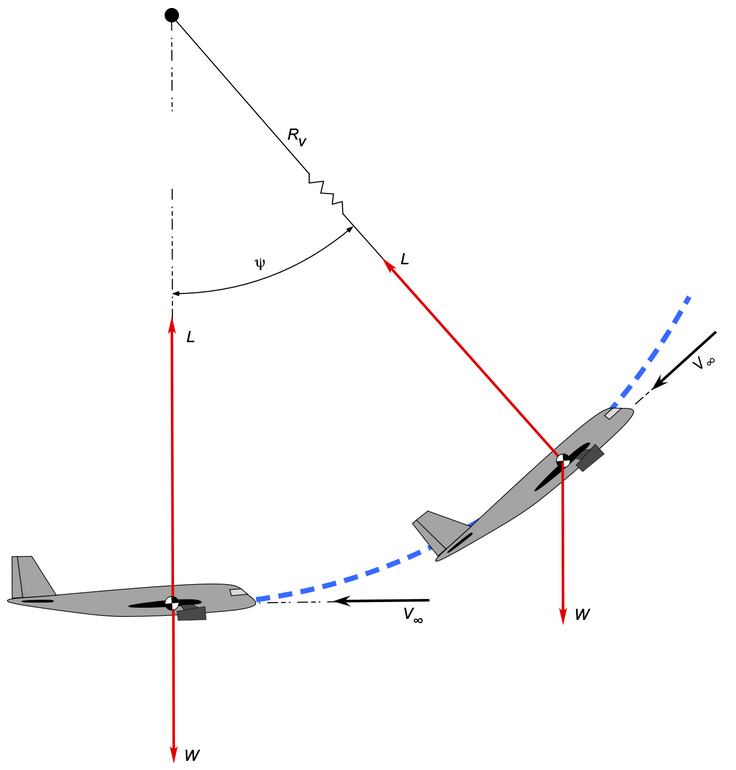
\includegraphics[width=.33\linewidth]{Imagens/img2_airPull.png}
        \caption{Somatório de forças em voo circular}
        \label{fig:enter-label}
    \end{figure}
\end{comment}